% consistency-theory.tex

%%%%%%%%%%%%%%%%%%%%%%%%%%%%%%
\begin{frame}{}
	\begin{center}
		\polysi{} 以黑盒的方式使用 MonoSAT 求解器

		\vspace{0.30cm}
		\fig{width = 0.70\textwidth}{figs/solver-blackbox}
		\vspace{0.30cm}

		未能充分利用 SAT/SMT 搜索框架 (DPLL/CDCL)
	\end{center}
\end{frame}
%%%%%%%%%%%%%%%%%%%%%%%%%%%%%%

%%%%%%%%%%%%%%%%%%%%%%%%%%%%%%
\begin{frame}{}
	\begin{center}
		\blue{\bf 当前的探索:} 如何``深度整合 SMT'', 进一步提升算法效率?

		\vspace{0.50cm}
		\fig{width = 0.70\textwidth}{figs/integrated}
	\end{center}
\end{frame}
%%%%%%%%%%%%%%%%%%%%%%%%%%%%%%

%%%%%%%%%%%%%%%%%%%%%%%%%%%%%%
\begin{frame}{}
	\begin{center}
		多线程程序验证问题~\ncite{Zord:PLDI2021}

		\vspace{0.30cm}
		\fig{width = 0.90\textwidth}{figs/pldi2021}
	\end{center}
\end{frame}
%%%%%%%%%%%%%%%%%%%%%%%%%%%%%%

%%%%%%%%%%%%%%%%%%%%%%%%%%%%%%
\begin{frame}{}
	\begin{center}
		设计专用的事务一致性理论求解器 (图片来自~\ncite{Zord:PLDI2021})

		\vspace{0.50cm}
		\fig{width = 0.65\textwidth}{figs/smt-framework}
	\end{center}
\end{frame}
%%%%%%%%%%%%%%%%%%%%%%%%%%%%%%

%%%%%%%%%%%%%%%%%%%%%%%%%%%%%%
\begin{frame}{}
	\fig{width = 0.95\textwidth}{figs/consistency-theory-solver-revised}

	%	\begin{itemize}
	%		\item \textcolor[RGB]{71,46,125}{\textbf{Pick}}: select a variable to make an assignment
	%		\item \textcolor[RGB]{71,46,125}{\textbf{T}}heory\textcolor[RGB]{71,46,125}{\textbf{-Propagate}}: efficiently detect possible cycle upon inserting arcs
	%		\item \textcolor[RGB]{71,46,125}{\textbf{T}}heory\textcolor[RGB]{71,46,125}{\textbf{-Analyze}}: find proper cycle(s)
	%		\item \textcolor[RGB]{71,46,125}{\textbf{Unit-edge Propagate}}: derive literatures from current reachability
	%	\end{itemize}
\end{frame}
%%%%%%%%%%%%%%%%%%%%%%%%%%%%%%

%%%%%%%%%%%%%%%%%%%%%%%%%%%%%%
\begin{frame}{}
	\begin{center}
		增量式环检测算法~\ncite{ICD:TOA2015} 与 Unit-edge Propagation

		\vspace{0.50cm}
		\fig{width = 0.95\textwidth}{figs/ICD-algorithm-and-unit-edge-propagation.png}
	\end{center}

	% takes at most $O(\min\{m^{1/2}, n^{2/3}\}m)$ time to insert $m$ arcs into an $n$-vertex graph.
\end{frame}
%%%%%%%%%%%%%%%%%%%%%%%%%%%%%%

%%%%%%%%%%%%%%%%%%%%%%%%%%%%%%
\begin{frame}{}{pruning, pair conflict generation, ...}
	\begin{center}
		剪枝: ``小环''占多数, 可以用于排除不可能的约束
	\end{center}

	\begin{figure}[H]
		\centering
		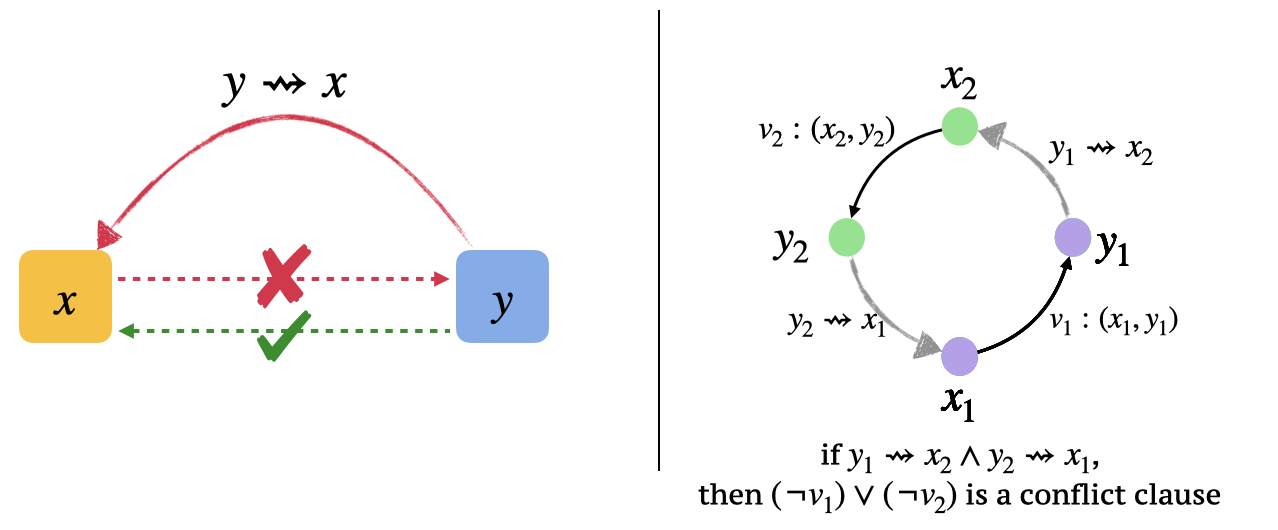
\includegraphics[width=0.9\textwidth]{figs/pruning-and-pair-conflict-generation.png}
	\end{figure}
\end{frame}
%%%%%%%%%%%%%%%%%%%%%%%%%%%%%%

%%%%%%%%%%%%%%%%%%%%%%%%%%%%%%
% \begin{frame}{}
% 	% \begin{center}
% 	% 	\scriptsize{
% 	% 		\begin{tabular}{|c|c|c|c|c|}
% 	% 			\hline
% 	% 			baseline & \makecell{cycle\\ detection} & \makecell{conflict\\ generation} & \makecell{unit-edge\\ propagation} & \makecell{pair conflict\\generation} \\
% 	% 			\hline
% 	% 			z3 user propagator* & local toposort & smallest & $\checkmark$(partial) & \\
% 	% 			\hline
% 	% 			monosat & PK toposort & first & & \\
% 	% 			\hline
% 	% 			acyclic minisat* & ICD & first & $\checkmark$ & $\checkmark$ \\
% 	% 			\hline
% 	% 			cobra(w/o GPU) & \multicolumn{3}{c|}{same as monosat} & \\
% 	% 			\hline
% 	% 		\end{tabular}
% 	% 	}
% 	% 	\\
% 	% 	\tiny{*: we implemented}
% 	% \end{center}

% 	\begin{figure}[H]
% 		\centering
% 		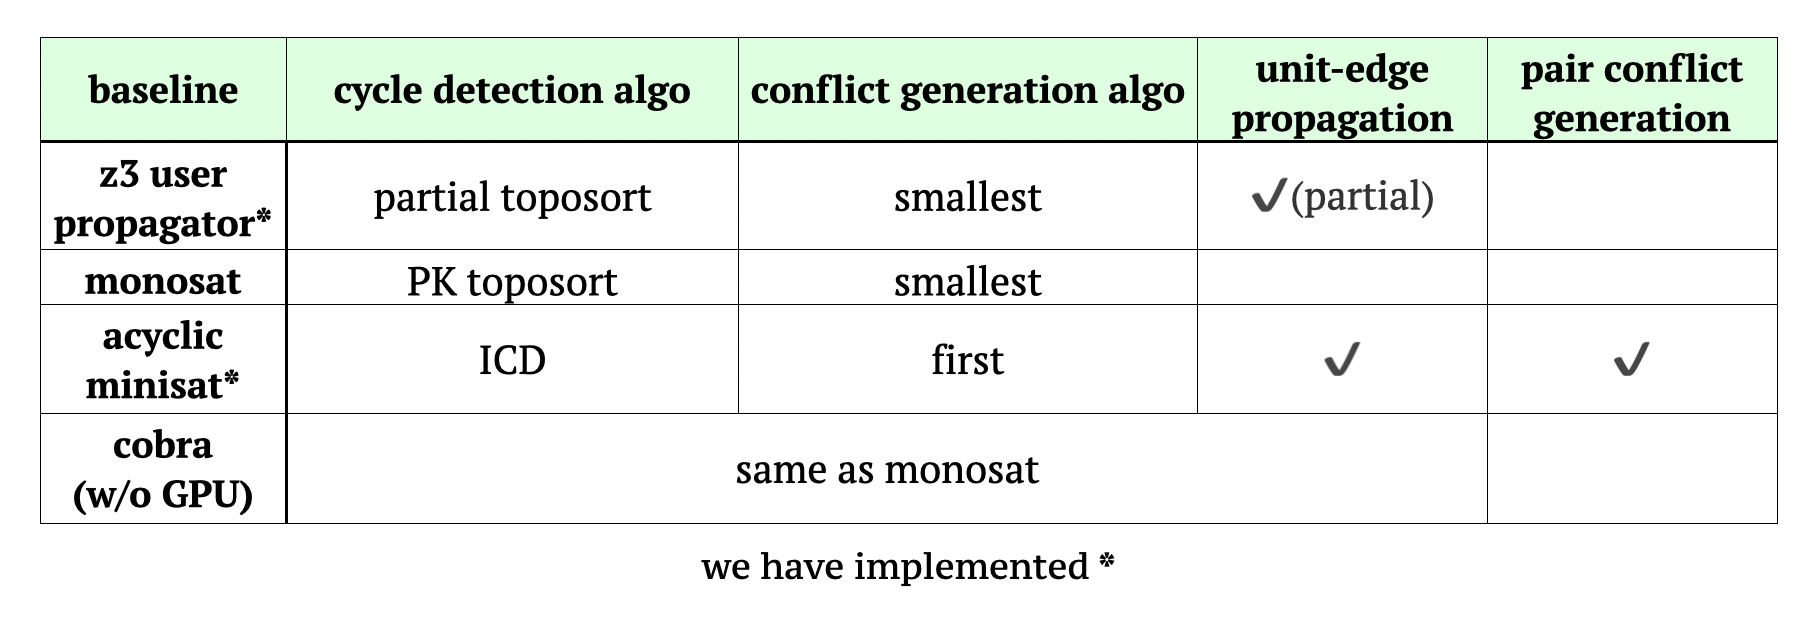
\includegraphics[width=\textwidth]{figs/ser-checker-baselines.png}
% 	\end{figure}
% \end{frame}
%%%%%%%%%%%%%%%%%%%%%%%%%%%%%%

%%%%%%%%%%%%%%%%%%%%%%%%%%%%%%
\begin{frame}{}
	\begin{center}
		``可序列化''一致性模型检测算法性能对比\blue{\bf 初步结果}
	\end{center}

	\begin{figure}[H]
		\centering
		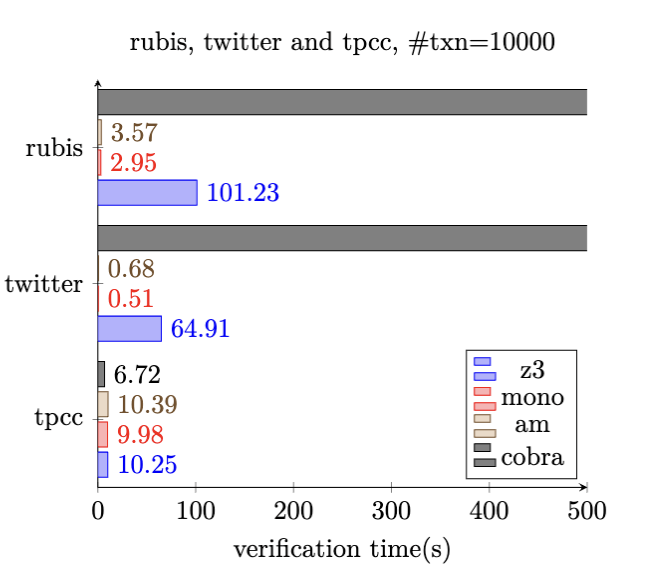
\includegraphics[width=0.48\textwidth]{figs/ser-checker-rubis-twitter-and-tpcc-ntxn10000.png}
		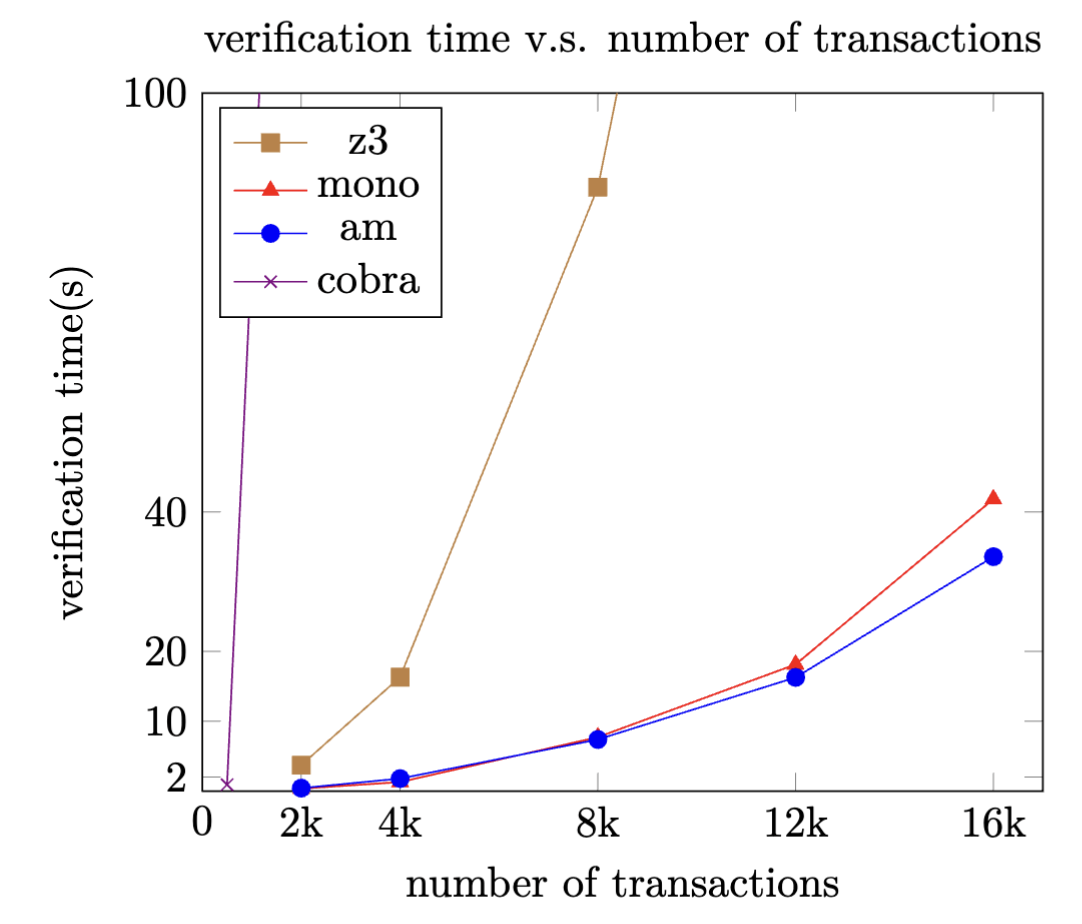
\includegraphics[width=0.48\textwidth]{figs/ser-checker-chengRW-verification-time-vs-ntxns.png}
	\end{figure}
\end{frame}
%%%%%%%%%%%%%%%%%%%%%%%%%%%%%%

% %%%%%%%%%%%%%%%%%%%%%%%%%%%%%%
% \begin{frame}{What Needs To Do Next}
% 	\begin{itemize}
% 		\item \textbf{pick}: leverage the underlying graph infomation to make a seemingly best assignment.
% 		\begin{itemize}
% 			\item to choose the variable that contains maximum / minimal edges, or is able to best trigger unit-edge propagation.
% 			\item to learn some infomation from those detected cycles.
% 		\end{itemize}
% 		\item \textbf{unify the approach to handle small width cycles}
% 		\begin{itemize}
% 			\item to design an algorithm that performs well on those small width cycles.
% 		\end{itemize}
% 		\item \textbf{make the theory solver lazier}
% 		\begin{itemize}
% 			\item observation: after pruning and pair conflict generation, the times of detecting a cycle has declined greatly.
% 			\item a lazier theory solver may be capable for big yet powerful cycle detection algorithms.
% 		\end{itemize}
% 	\end{itemize}
% \end{frame}
% %%%%%%%%%%%%%%%%%%%%%%%%%%%%%%